\documentclass{article}
\pagestyle{empty}

\usepackage[papersize={5.5in,3.5in}, margin=0.2in, marginratio=1:1]{geometry}

\usepackage{graphicx}        % ����ͼƬ
\usepackage{xcolor}          % ����������ɫ
\usepackage{background}      % ����ҳ�汳��ͼ��
\usepackage{noto}
\usepackage{xeCJK}
\usepackage{amsmath}
\usepackage{latexsym}
\usepackage{tabularx}
\usepackage{metalogo}
\usepackage{ulem}
\renewcommand{\quad}{\hspace*{2.5ex}}
\setlength{\parindent}{0pt}
\renewcommand{\familydefault}{\sfdefault}
\newcolumntype{Y}{>{\centering\arraybackslash}X}
\newcommand{\balancedVPhantom}[1]{% gives minimum vertical size
  $\mathsurround=0pt \vcenter{\hrule width0pt height #1}$\ignorespaces
}

% ���ñ���ͼ
\backgroundsetup{
  scale=1,
  angle=0,
  opacity=1,
  contents={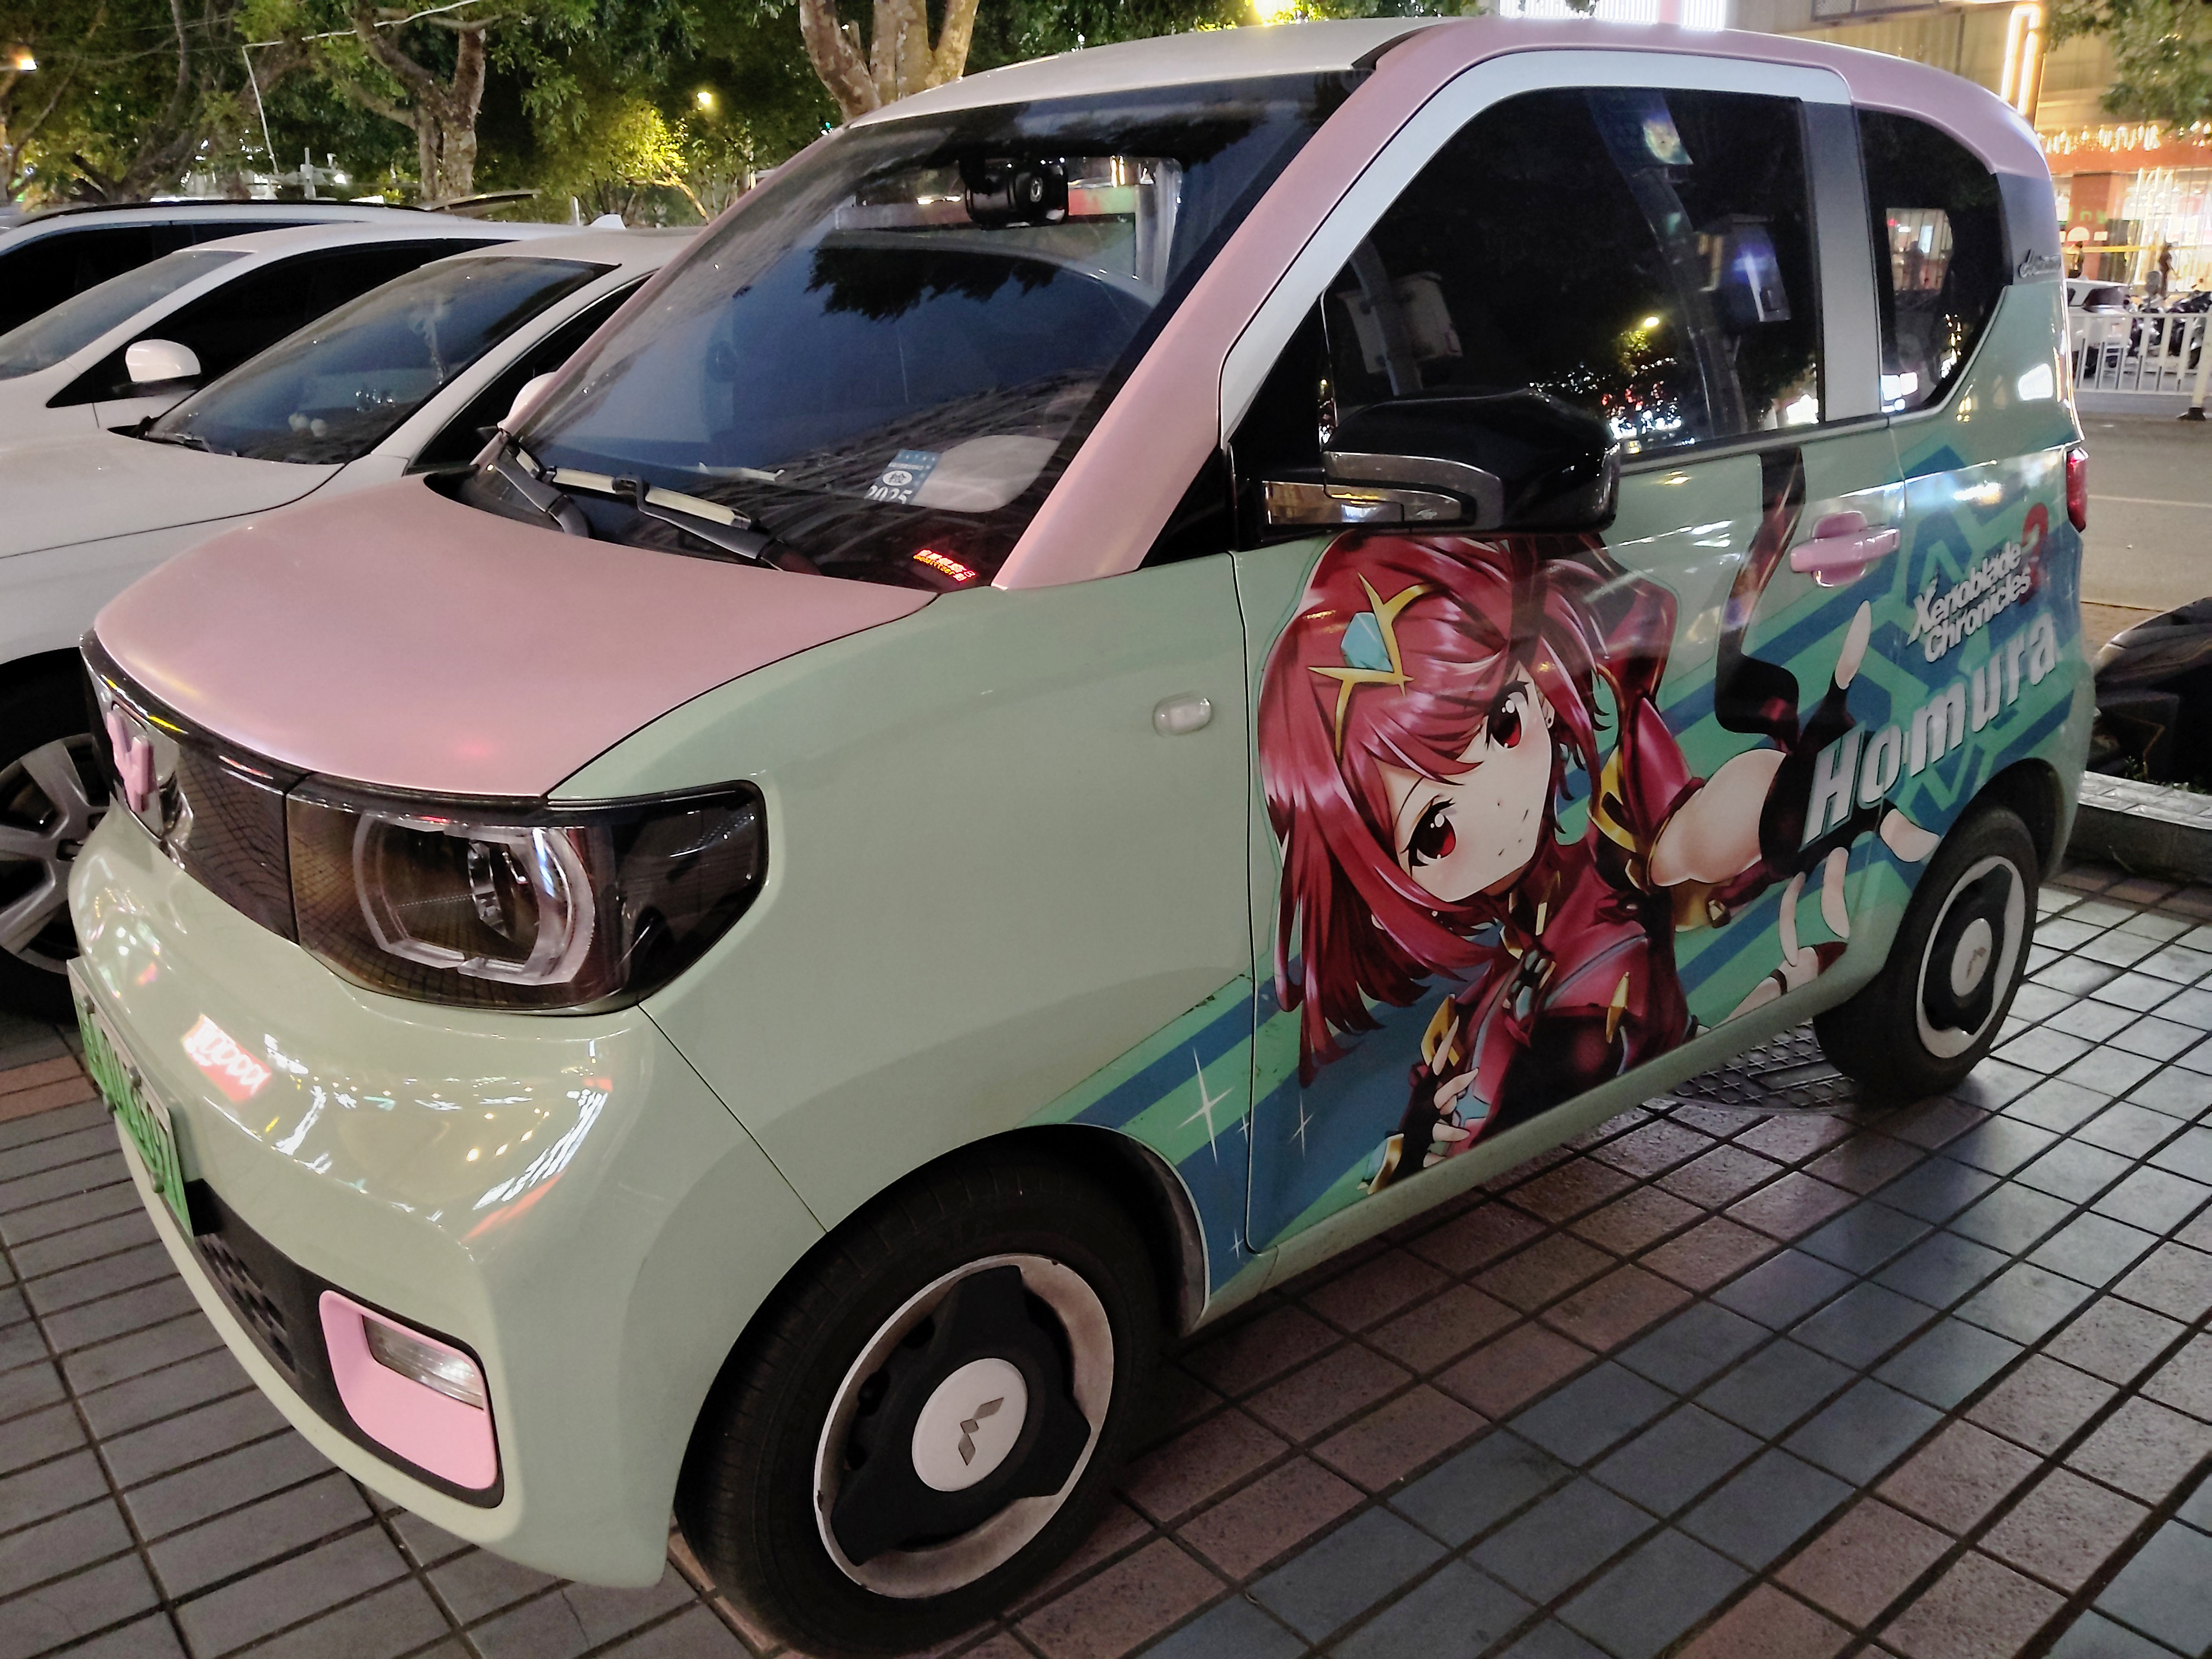
\includegraphics[width=\paperwidth,height=\paperheight]{images/front.jpg}}
}

% ������������Ϊ��ɫ
\color{white}

\begin{document}
\begin{minipage}{\textwidth}
    \centering {\Huge \textcolor{red}{\texttt{\textbf{BG7XTQ}}}}
\end{minipage}

\vfill

\begin{minipage}[t]{0.3\textwidth}
    \textbf{Funing Mo} \\
    \footnotesize
    1 Dong 1 Danyuan 302 \\
    Qixing Lu 133 Hao, Qingxiu Qu \\
    Nanning, Guangxi 530012 \\
    People's Republic of China
\end{minipage}
\begin{minipage}[t]{0.35\textwidth}
    \begin{footnotesize}
        \begin{tabbing}
            ITU Zone:
                \=  00
                \=  00
                \kill
            CQ Zone:
                \>  24 \,
                \>  \\
            ITU Zone:
                \>  43 \,
                \>  \\
        \end{tabbing}
    \end{footnotesize}
\end{minipage}
\hfill
\begin{minipage}[t]{0.35\textwidth}
    \centering
    \scriptsize
    \framebox[\textwidth][l]{\scriptsize Confirming QSO with: \texttt{BG7ABC} \vphantom{$\int\limits_{\dfrac aa}$}}
\end{minipage}
\vfill
\begin{minipage}{\textwidth}
    \footnotesize Confirming the following:
    \topsep3pt
    \begin{center}
        \begin{tabularx}{\textwidth}{|Y|Y|Y|Y|Y|c|c|c|}
            \hline
            \rule{0pt}{0.125in}\textbf{Day} & \textbf{Month} & \textbf{Year} & \textbf{UTC} & \textbf{MHz} & \,\,\, \textbf{Mode} \,\,\, & \,\,\, \textbf{RST} \,\,\, & \textbf{QSL} \\
            \hline
            \hline
			 \balancedVPhantom{2em} & XXX & 2025 & 1234 & 433.000 & FM & 59 & PSE \; \sout{TNX} \\
            \hline
        \end{tabularx}
    \end{center}
\end{minipage}

\vfill

\footnotesize \textbf{GRID:} \texttt{AB12cd}
\vfill

\footnotesize \textbf{Rig:} Device \makebox[0.3\textwidth]{} \textbf{Power:} 0W \makebox[0.1\textwidth]{} \textbf{Comments:}

\vfill

\footnotesize \textbf{Previous call sign held:} \texttt{JJ1DSB}

\vfill

\textbf{Antenna:} Antenna \makebox[1cm]{}

\vfill

\tiny
\end{document}
